\documentclass[journal]{IEEEtai}

\usepackage[colorlinks,urlcolor=blue,linkcolor=blue,citecolor=blue]{hyperref}
\usepackage[UTF8]{ctex} 
\usepackage{color,array}

\usepackage{graphicx}

%% \jvol{XX}
%% \jnum{XX}
%% \paper{1234567}
%% \pubyear{2020}
%% \publisheddate{xxxx 00, 0000}
%% \currentdate{xxxx 00, 0000}
%% \doiinfo{TQE.2020.Doi Number}

\newtheorem{theorem}{Theorem}
\newtheorem{lemma}{Lemma}
\setcounter{page}{1}
%% \setcounter{secnumdepth}{0}
\bibliographystyle{elsarticle-num}
\usepackage[numbers,sort,compress]{natbib}
\begin{document}


\title{基于深度学习的时间序列预测 (December 2021)} 


\author{张威伦, \IEEEmembership{南昌大学, 信息工程学院}, 黄晴楠,张敏,高彤, 和 饶旺, \IEEEmembership{南昌大学, 信息工程学院}
\thanks{This paragraph of the first footnote will contain the date on which you submitted your paper for review. It will also contain support information, including sponsor and financial support acknowledgment. For example, ``This work was supported in part by the U.S. Department of Commerce under Grant BS123456.'' }
\thanks{The next few paragraphs should contain the authors' current affiliations, including current address and e-mail. For example, F. A. Author is with the National Institute of Standards and Technology, Boulder, CO 80305 USA (e-mail: author@boulder.nist.gov).}
\thanks{S. B. Author, Jr., was with Rice University, Houston, TX 77005 USA. He is now with the Department of Physics, Colorado State University, Fort Collins, CO 80523 USA (e-mail: author@lamar.colostate.edu).}
\thanks{T. C. Author is with the Electrical Engineering Department, University of Colorado, Boulder, CO 80309 USA, on leave from the National Research Institute for Metals, Tsukuba, Japan (e-mail: author@nrim.go.jp).}
\thanks{This paragraph will include the Associate Editor who handled your paper.}}

\markboth{Journal of IEEE Transactions on Artificial Intelligence, Vol. 00, No. 0, Month 2020}
{First A. Author \MakeLowercase{\textit{et al.}}: Bare Demo of IEEEtai.cls for IEEE Journals of IEEE Transactions on Artificial Intelligence}

\maketitle

\begin{abstract}
	 天气对人的劳作和生产都会产生或多或少的影响,同时它也会影响经济发展和环境变化,通过物理模型我们可以预测短期内的天气状况,而如何通过总结天气变化的规律,从而预测气象是一个很重要的课题。伴随着计算机技术的迅猛发展,深度学习在生活中越来越多地被应用,深度学习在计算机视觉、语音识别、自然语言处理等领域取得的突破性进展,新技术创新带来的不仅是挑战,同时也给气象预测技术的发展带来了机遇。在\cite{schultz2021can}中,作者研究了用深度学习方法预测数字化的天气,其使用了NWP-DL模型进行预测。在\cite{ahyar2020firefly}中,作者使用了循环神经网络Deep Recurrent Neural Networks(DRNN)对天气预测进行研究,他尝试了不同的学习率,优化器,最终得到了比较低的错误率。

	本课题研究基于深度学习的时间序列预测,针对气象温度进行时间序列建模,通过分析国内外研究现状及对时间序列预测模型的研究与对比,研究如何通过时间序列进行气象预测,我们将使用深度学习方法,基于循环神经网络对天气进行预测,用RSE、MSE进行损失计算,从而找到最优的模型。
	\nocite{*}
\end{abstract}







\section{介绍}

\IEEEPARstart{T}{his} document is a template for Microsoft {\it Word} versions 6.0 or later. If you are reading a paper or PDF version of this document, please download the electronic file, trans\_jour.docx, from the IEEE Web site at \href{http://www.ieee.org/authortools}{www.ieee.org/authortools} so you can use it to prepare your manuscript. If you would prefer to use \LaTeX, download IEEE's  {\LaTeX} style and sample files from the same Web page. You can also explore using the Overleaf editor at {https://www.overleaf.com/blog/278-how-to-use-overleaf-with-ieee-collabratec-your-quick-guide-to-getting-started\#.Vp6tpPkrKM9}

If your paper is intended for a conference, please contact your conference editor concerning acceptable word processor formats for your particular conference.

\section{Guidelines for Manuscript Preparation}

When you open trans\_jour.docx, select ``Page Layout'' from the ``View'' menu in the menu bar (View $|$ Page Layout), (these instructions assume MS 6.0. Some versions may have alternate ways to access the same functionalities noted here). Then, type over sections of trans\_jour.docx or cut and paste from another document and use markup styles. The pull-down style menu is at the left of the Formatting Toolbar at the top of your {\it Word} window (for example, the style at this point in the document is ``Text''). Highlight a section that you want to designate with a certain style, and then select the appropriate name on the style menu. The style will adjust your fonts and line spacing. Do not change the font sizes or line spacing to squeeze more text into a limited number of pages. Use italics for emphasis; do not underline.

To insert images in {\it Word}, position the cursor at the insertion point and either use Insert $|$ Picture $|$ From File or copy the image to the Windows clipboard and then Edit $|$ Paste Special $|$ Picture (with ``float over text'' unchecked). 

IEEE will do the final formatting of your paper. If your paper is intended for a conference, please observe the conference page limits.

\subsection{Abbreviations and Acronyms}

Define abbreviations and acronyms the first time they are used in the text, even after they have already been defined in the abstract. Abbreviations such as IEEE, SI, ac, and dc do not have to be defined. Abbreviations that incorporate periods should not have spaces: write ``C.N.R.S.,'' not ``C. N. R. S.'' Do not use abbreviations in the title unless they are unavoidable (for example, ``IEEE'' in the title of this article).

\subsection{Other Recommendations}

Use one space after periods and colons. Hyphenate complex modifiers: ``zero-field-cooled magnetization.'' Avoid dangling participles, such as, ``Using (1), the potential was calculated.'' [It is not clear who or what used (1).] Write instead, ``The potential was calculated by using (1),'' or ``Using (1), we calculated the potential.''

Use a zero before decimal points: ``0.25,'' not ``.25.'' Use ``cm$^3$,'' not ``cc.'' Indicate sample dimensions as ``0.1~cm~$\times$ 0.2 cm,'' not ``0.1 $\times$ 0.2 cm$^2$.'' The abbreviation for ``seconds'' is ``s,'' not ``sec.'' Use ``Wb/m$^2$'' or ``webers per square meter,'' not ``webers/m$^2$.'' When expressing a range of values, write ``7 to 9'' or ``7-9,'' not ``7$\sim$9.''

A parenthetical statement at the end of a sentence is punctuated outside of the closing parenthesis (like this). (A parenthetical sentence is punctuated within the parentheses.) In American English, periods and commas are within quotation marks, like ``this period.'' Other punctuation is ``outside''$!$ Avoid contractions; for example, write ``do not'' instead of ``don't.'' The serial comma is preferred: ``A, B, and C'' instead of ``A, B and C.''

If you wish, you may write in the first person singular or plural and use the active voice (``I observed that ...'' or ``We observed that ...'' instead of ``It was observed that ...''). Remember to check spelling. If your native language is not English, please get a native English-speaking colleague to carefully proofread your paper.

\section{Math}

If you are using {\it Word}, use either the Microsoft Equation Editor or the {\it MathType} add-on (http://www.mathtype.com) for equations in your paper (Insert $|$ Object $|$ Create New $|$ Microsoft Equation {\it or} MathType Equation). ``Float over text'' should {\it not} be selected.

\subsection{Equations}

Number equations consecutively with equation numbers in parentheses flush with the right margin, as in (1). First use the equation editor to create the equation. Then select the ``Equation'' markup style. Press the tab key and write the equation number in parentheses. To make your equations more compact, you may use the solidus ( / ), the exp function, or appropriate exponents. Use parentheses to avoid ambiguities in denominators. Punctuate equations when they are part of a sentence, as in
\begin{equation}
\!
\end{equation}
Be sure that the symbols in your equation have been defined before the equation appears or immediately following. Italicize symbols ($T$ might refer to temperature, but T is the unit tesla). Refer to ``(1),'' not ``Eq. (1)'' or ``equation~(1),'' except at the beginning of a sentence: ``Equation (1) is ....''


\section{Units}

Use either SI (MKS) or CGS as primary units. (SI units are strongly encouraged.) English units may be used as secondary units (in parentheses). This applies to papers in data storage. For example, write ``15 Gb/cm$^2$ (100 Gb/in$^2$).'' An exception is when English units are used as identifiers in trade, such as ``3$^1${/}$_2$-in disk drive.'' Avoid combining SI and CGS units, such as current in amperes and magnetic field in oersteds. This often leads to confusion because equations do not balance dimensionally. If you must use mixed units, clearly state the units for each quantity in an equation.

The SI unit for magnetic field strength $H$ is A/m. However, if you wish to use units of T, either refer to magnetic flux density $B$ or magnetic field strength symbolized as $\mu_0$H. Use the center dot to separate compound units, e.g., ``A$\cdot$m$^2$.''

\section{Some Common Mistakes}

The word ``data'' is plural, not singular. The subscript for the permeability of vacuum $\mu_0$ is zero, not a lowercase letter ``o.'' The term for residual magnetization is ``remanence''; the adjective is ``remanent''; do not write ``remnance'' or ``remnant.'' Use the word ``micrometer'' instead of ``micron.'' A graph within a graph is an ``inset,'' not an ``insert.'' The word ``alternatively'' is preferred to the word ``alternately'' (unless you really mean something that alternates). Use the word ``whereas'' instead of ``while'' (unless you are referring to simultaneous events). Do not use the word ``essentially'' to mean ``approximately'' or ``effectively.'' Do not use the word ``issue'' as a euphemism for ``problem.'' When compositions are not specified, separate chemical symbols by en-dashes; for example, ``NiMn'' indicates the intermetallic compound Ni$_{0.5}$Mn$_{0.5}$ whereas ``Ni--Mn'' indicates an alloy of some composition Ni$_{\rm x}$Mn$_{1-{\rm x}}$.

Be aware of the different meanings of the homophones ``affect'' (usually a verb) and ``effect'' (usually a noun), ``complement'' and ``compliment,'' ``discreet'' and ``discrete,'' ``principal'' (e.g., ``principal investigator'') and ``principle'' (e.g., ``principle of measurement''). Do not confuse ``imply'' and\break ``infer.'' 

Prefixes such as ``non,'' ``sub,'' ``micro,'' ``multi,'' and ``ultra'' are not independent words; they should be joined to the words they modify, usually without a hyphen. There is no period after the ``et'' in the Latin abbreviation ``{\it et al}.'' (it is also italicized). The abbreviation ``i.e.,'' means ``that is,'' and the abbreviation ``e.g.,'' means ``for example'' (these abbreviations are not italicized).

A general IEEE styleguide is available at www.ieee.org/authortools.

\section{Guidelines For Graphics Preparation and Submission}

\subsection{Types of Graphics}

The following list outlines the different types of graphics published in IEEE journals. They are categorized based on their construction, and use of color / shades\vadjust{\pagebreak} of gray:

\begin{enumerate}
\item[{\it 1)}]{\it Color/Grayscale Figures}

Figures that are meant to appear in color, or shades of black/gray. Such figures may include photographs, illustrations, multicolor graphs, and flowcharts.

\item[{\it 2)}]{\it Line Art Figures}

Figures that are composed of only black lines and shapes. These figures should have no shades or half-tones of gray, only black and white.

\item[{\it 3)}]{\it Author Photos}

Head and shoulders shots of authors that appear at the end of our papers.

\item[{\it 4)}]{\it Tables}

Data charts which are typically black and white, but sometimes include color.
\end{enumerate}
\begin{figure}
\centerline{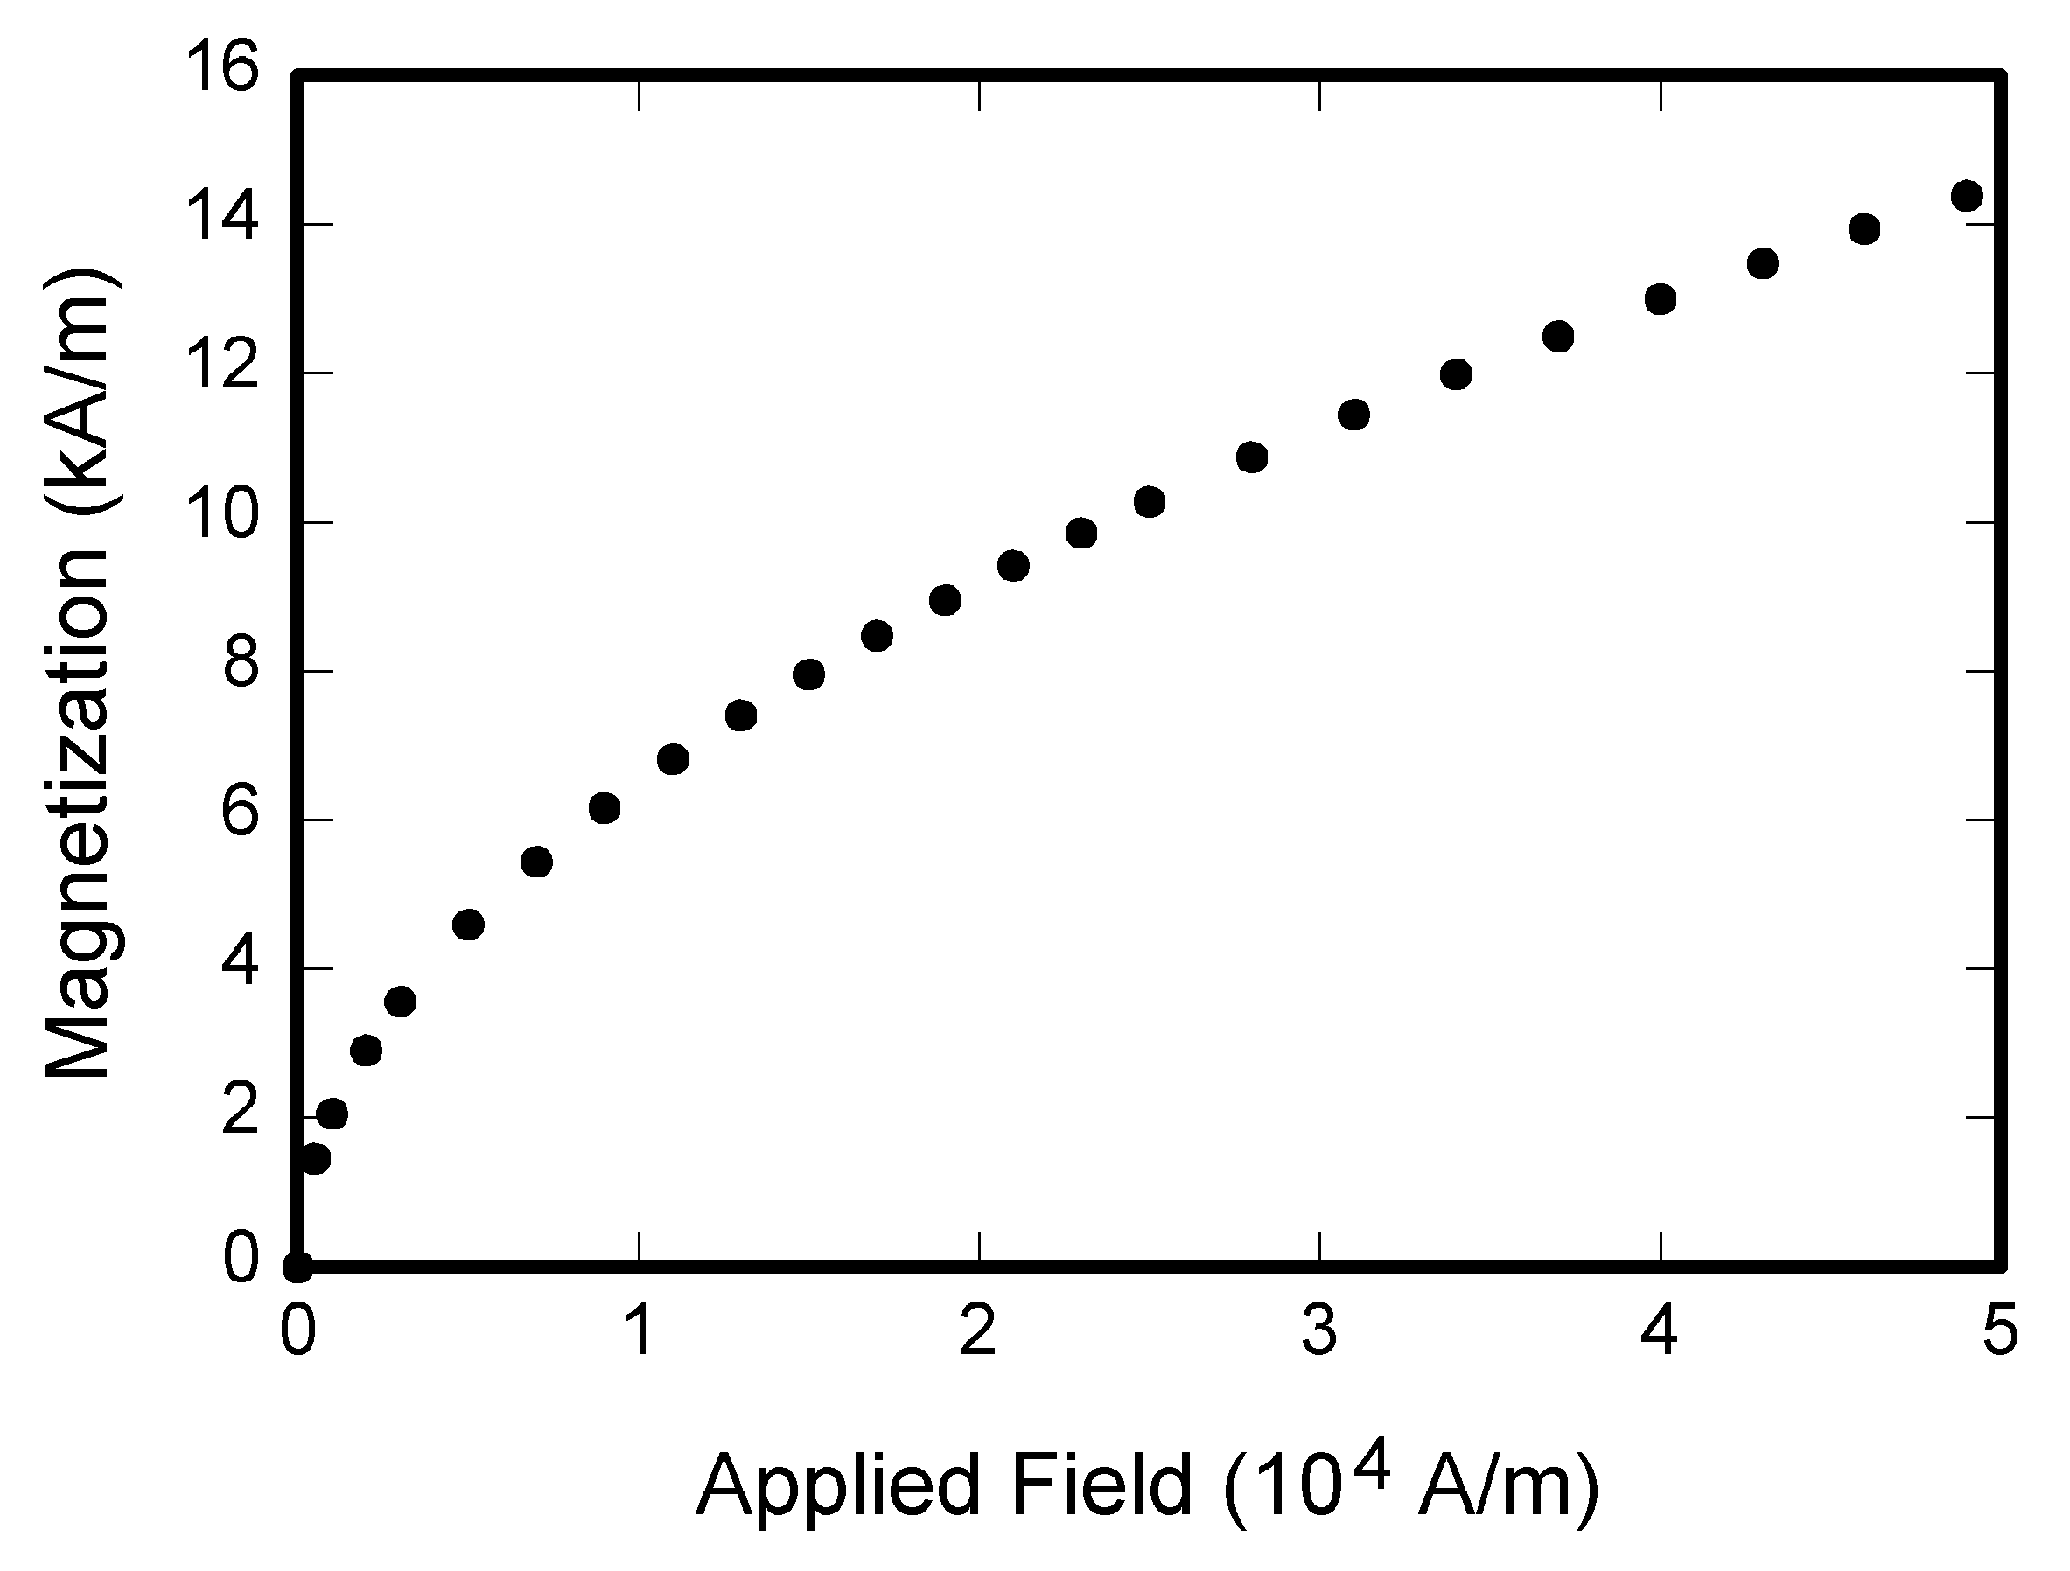
\includegraphics[width=18.5pc]{fig1.png}}
\caption{Magnetization as a function of applied field. Note that ``Fig.'' is abbreviated. There is a period after the figure number, followed by two spaces. It is good practice to explain the significance of the figure in the caption.}
\end{figure}

\begin{table}
\caption{Units for Magnetic Properties}
\label{table}
\tablefont%
\setlength{\tabcolsep}{3pt}
\begin{tabular*}{21pc}{@{}|p{23pt}|p{81pt}<{\raggedright\hangindent6pt}|p{123pt}<{\raggedright\hangindent6pt}|@{}}
\hline
Symbol& 
Quantity& 
Conversion from Gaussian and \par CGS EMU to SI$^{\mathrm{a}}$ \\
\hline\\[-17pt]
&&\\
$\Phi $& 
Magnetic flux& 
1 Mx $\to  10^{-8}$ Wb $= 10^{-8}$ V$\,\cdot\,$s \\
$B$& 
Magnetic flux density, magnetic induction& 
1 G $\to  10^{-4}$ T $= 10^{-4}$~Wb/m$^{2}$ \\
$H$& 
Magnetic field strength& 
1 Oe $\to  10^{-3}/(4\pi )$ A/m \\
$m$& 
Magnetic moment& 
1 erg/G $=$ 1 emu\\ && $\to 10^{-3}$ A $\cdot$ m$^{2} = 10^{-3}$ J/T \\
$M$& 
Magnetization& 
1 erg/(G $\cdot$ cm$^{3}) =$ 1 emu/cm$^{3}$  $\to 10^{-3}$ A/m \\
4$\pi M$& 
Magnetization& 
1 G $\to  10^{-3}/(4\pi )$ A/m \\
$\sigma $& 
Specific magnetization& 
1~erg/(G$\,{\cdot}\,$g)$\,{=}\,$1~emu/g$\,{\to}\,$1~A$\,{\cdot}\,$m$^{2}$/kg \\
$j$& 
Magnetic dipole  moment& 
1 erg/G $=$ 1 emu\par $\to 4\pi \times  10^{-10}$ Wb $\cdot$ m \\
$J$& 
Magnetic polarization& 
1 erg/(G $\cdot$ cm$^{3}) =$ 1 emu/cm$^{3}$ \\ && $\to 4\pi \times  10^{-4}$ T \\
$\chi , \kappa $& 
Susceptibility& 
1 $\to  4\pi $ \\
$\chi_{\rho }$& 
Mass susceptibility& 
1 cm$^{3}$/g $\to  4\pi \times  10^{-3}$ m$^{3}$/kg \\
$\mu $& 
Permeability& 
1 $\to  4\pi \times  10^{-7}$ H/m\par  $= 4\pi \times  10^{-7}$ Wb/(A $\cdot$ m) \\
$\mu_{r}$& 
Relative permeability& 
$\mu \to \mu_{r}$ \\
$w, W$& 
Energy density& 
1 erg/cm$^{3} \to  10^{-1}$ J/m$^{3}$ \\
$N, D$& 
Demagnetizing factor& 
1 $\to  1/(4\pi )$ \\
\hline
\multicolumn{3}{l}{}\\[-5pt]
\multicolumn{3}{@{}p{21pc}@{}}{\hspace*{9pt}Vertical lines are optional in tables. Statements that serve as captions for 
the entire table do not need footnote letters. }\\
\multicolumn{3}{@{}p{21pc}@{}}{\hspace*{9pt}$^{\mathrm{a}}$Gaussian units are the same as cg emu for magnetostatics; Mx 
$=$ maxwell, G $=$ gauss, Oe $=$ oersted; Wb $=$ weber, V $=$ volt, s $=$ 
second, T $=$ tesla, m $=$ meter, A $=$ ampere, J $=$ joule, kg $=$ 
kilogram, H $=$ henry.}
\end{tabular*}
\label{tab1}
\end{table}



\subsection{Multipart Figures}

Figures compiled of more than one sub-figure presented side-by-side, or stacked. If a multipart figure is made up of multiple figure types (one part is lineart, and another is grayscale or color) the figure should meet the stricter guidelines.

\subsection{File Formats for Graphics}

Format and save your graphics using a suitable graphics processing program that will allow you to create the images as PostScript (PS), Encapsulated PostScript (.EPS), Tagged Image File Format (.TIFF), Portable Document Format (.PDF), or Portable Network Graphics (.PNG) sizes them, and adjusts the resolution settings. If you created your source files in one of the following programs you will be able to submit the graphics without converting to a PS, EPS, TIFF, PDF, or PNG file: Microsoft Word, Microsoft PowerPoint, or Microsoft Excel. Though it is not required, it is strongly recommended that these files be saved in PDF format rather than DOC, XLS, or PPT. Doing so will protect your figures from common font and arrow stroke issues that occur when working on the files across multiple platforms. When submitting your final paper, your graphics should all be submitted individually in one of these formats along with the manuscript.


\subsection{Sizing of Graphics}

Most charts, graphs, and tables are one column wide (3.5 inches / 88 millimeters / 21 picas) or page wide (7.16 inches / 181 millimeters / 43 picas). The maximum depth a graphic can be is 8.5 inches (216 millimeters / 54 picas). When choosing the depth of a graphic, please allow space for a caption. Figures can be sized between column and page widths if the author chooses, however it is recommended that figures are not sized less than column width unless when necessary.

There is currently one publication with column measurements that do not coincide with those listed above. Proceedings of the IEEE has a column measurement of 3.25 inches (82.5 millimeters / 19.5 picas). 

The final printed size of author photographs is exactly 1 inch wide by 1.25 inches tall (25.4 millimeters $\times$ 31.75 millimeters / 6 picas $\times$ 7.5 picas). Author photos printed in editorials measure 1.59 inches wide by 2 inches tall (40 millimeters $\times$ 50 millimeters / 9.5 picas $\times$ 12 picas).

\subsection{Resolution}

The proper resolution of your figures will depend on the type of figure it is as defined in the ``Types of Figures'' section. Author photographs, color, and grayscale figures should be at least 300dpi. Line art, including tables should be a minimum of 600dpi.

\subsection{Vector Art}

In order to preserve the figures' integrity across multiple computer platforms, we accept files in the following formats: .EPS/.PDF/.PS. All fonts must be embedded or text converted to outlines in order to achieve the best-quality results.

\subsection{Color Space}

The term color space refers to the entire sum of colors that can be represented within the said medium. For our purposes, the three main color spaces are Grayscale, RGB (red/green/blue) and CMYK (cyan/magenta/yellow/black). RGB is generally used with on-screen graphics, whereas CMYK is used for printing purposes.

All color figures should be generated in RGB or CMYK color space. Grayscale images should be submitted in Grayscale color space. Line art may be provided in grayscale OR bitmap colorspace. Note that ``bitmap colorspace'' and ``bitmap file format'' are not the same thing. When bitmap color space is selected, .TIF/.TIFF/.PNG are the recommended file formats.

\subsection{Accepted Fonts Within Figures}

When preparing your graphics IEEE suggests that you use of one of the following Open Type fonts: Times New Roman, Helvetica, Arial, Cambria, and Symbol. If you are supplying EPS, PS, or PDF files all fonts must be embedded. Some fonts may only be native to your operating system; without the fonts embedded, parts of the graphic may be distorted or missing.

A safe option when finalizing your figures is to strip out the fonts before you save the files, creating ``outline'' type. This converts fonts to artwork what will appear uniformly on any screen.

\subsection{Using Labels Within Figures}

\subsubsection{Figure Axis Labels}

Figure axis labels are often a source of confusion. Use words rather than symbols. As an example, write the quantity ``Magnetization,'' or ``Magnetization $M$,'' not just ``$M$.'' Put units in parentheses. Do not label axes only with units. As in Fig. 1, for example, write ``Magnetization (A/m)'' or ``Magnetization (A$\cdot$m$^{-1}$),'' not just ``A/m.'' Do not label axes with a ratio of quantities and units. For example, write ``Temperature (K),'' not ``Temperature/K.''
 
Multipliers can be especially confusing. Write ``Magnetization (kA/m)'' or ``Magnetization (10$^3$ A/m).'' Do not write ``Magnetization (A/m) $\times$ 1000'' because the reader would not know whether the top axis label in Fig. 1 meant 16000 A/m or 0.016 A/m. Figure labels should be legible, approximately 8 to 10 point type.

\subsubsection{Subfigure Labels in Multipart Figures and Tables}

Multipart figures should be combined and labeled before final submission. Labels should appear centered below each subfigure in 8 point Times New Roman font in the format of (a) (b) (c). 

\subsection{File Naming}

Figures (line artwork or photographs) should be named starting with the first 5 letters of the author’s last name. The next characters in the filename should be the number that represents the sequential location of this image in your article. For example, in author ``Anderson's'' paper, the first three figures would be named ander1.tif, ander2.tif, and ander3.ps.

Tables should contain only the body of the table (not the caption) and should be named similarly to figures, except that `.t' is inserted in-between the author's name and the table number. For example, author Anderson's first three tables would be named ander.t1.tif, ander.t2.ps, ander.t3.eps.

Author photographs should be named using the first five characters of the pictured author's last name. For example, four author photographs for a paper may be named: oppen.ps, moshc.tif, chen.eps, and duran.pdf.

If two authors or more have the same last name, their first initial(s) can be substituted for the fifth, fourth, third... letters of their surname until the degree where there is differentiation. For example, two authors Michael and Monica Oppenheimer's photos would be named oppmi.tif, and oppmo.eps.

\subsection{Referencing a Figure or Table Within Your Paper}
 
When referencing your figures and tables within your paper, use the abbreviation ``Fig.'' even at the beginning of a sentence. Do not abbreviate ``Table.'' Tables should be numbered with Roman Numerals.

\subsection{Checking Your Figures: The IEEE Graphics Analyzer}

The IEEE Graphics Analyzer enables authors to pre-screen their graphics for compliance with IEEE Transactions and Journals standards before submission. The online tool, located at \underline{http://graphicsqc.ieee.org/}, allows authors to upload their graphics in order to check that each file is the correct file format, resolution, size and colorspace; that no fonts are missing or corrupt; that figures are not compiled in layers or have transparency, and that they are named according to the IEEE Transactions and Journals naming convention. At the end of this automated process, authors are provided with a detailed report on each graphic within the web applet, as well as by email.

For more information on using the Graphics Analyzer or any other graphics related topic, contact the IEEE Graphics Help Desk by e-mail at \underline{graphics@ieee.org}.

\subsection{Submitting Your Graphics}

Because IEEE will do the final formatting of your paper, you do not need to position figures and tables at the top and bottom of each column. In fact, all figures, figure captions, and tables can be placed at the end of your paper. In addition to, or even in lieu of submitting figures within your final manuscript, figures should be submitted individually, separate from the manuscript in one of the file formats listed above in section VI-J. Place figure captions below the figures; place table titles above the tables. Please do not include captions as part of the figures, or put them in ``text boxes'' linked to the figures. Also, do not place borders around the outside of your figures.


\subsection{Color Processing / Printing in IEEE Journals}

All IEEE Transactions, Journals, and Letters allow an author to publish color figures on IEEE {\it Xplore}$^{\scriptsize\textregistered}$ at no charge, and automatically convert them to grayscale for print versions. In most journals, figures and tables may alternatively be printed in color if an author chooses to do so. Please note that this service comes at an extra expense to the author. If you intend to have print color graphics, include a note with your final paper indicating which figures or tables you would like to be handled that way, and stating that you are willing to pay the additional fee.

\section{Conclusion}

A conclusion section is not required. Although a conclusion may review the main points of the paper, do not replicate the abstract as the conclusion. A conclusion might elaborate on the importance of the work or suggest applications and extensions.

\section*{Appendix}

Appendixes, if needed, appear before the acknowledgment.

\section*{Acknowledgment}

The preferred spelling of the word ``acknowledgment'' in American English is without an ``e'' after the ``g.'' Use the singular heading even if you have many acknowledgments. Avoid expressions such as ``One of us (S.B.A.) would like to thank ... .'' Instead, write ``F. A. Author thanks ... .'' In most cases, sponsor and financial support acknowledgments are placed in the unnumbered footnote on the first page, not here.

\section*{References and Footnotes}

\subsection{References}

References need not be cited in text. When they are, they appear on the line, in square brackets, inside the punctuation. Multiple references are each numbered with separate brackets. When citing a section in a book, please give the relevant page numbers. In text, refer simply to the reference number. Do not use ``Ref.'' or ``reference'' except at the beginning of a sentence: ``Reference [3] shows~....'' Please do not use automatic endnotes in {\it Word}, rather, type the reference list at the end of the paper using the ``References''  style.

Reference numbers are set flush left and form a column of their own, hanging out beyond the body of the reference. The reference numbers are on the line, enclosed in square brackets. In all references, the given name of the author or editor is abbreviated to the initial only and precedes the last name. Use them all; use {\it et al}. only if names are not given. Use commas around Jr., Sr., and III in names. Abbreviate conference titles. When citing IEEE transactions, provide the issue number, page range, volume number, year, and/or month if available. When referencing a patent, provide the day and the month of issue, or application. References may not include all information; please obtain and include relevant information. Do not combine references. There must be only one reference with each number. If there is a URL included with the print reference, it can be included at the end of the reference. 

Other than books, capitalize only the first word in a paper title, except for proper nouns and element symbols. For papers published in translation journals, please give the English citation first, followed by the original foreign-language citation See the end of this document for formats and examples of common references. For a complete discussion of references and their formats, see the IEEE style manual at \underline{www.ieee.org/authortools}.

\subsection{Footnotes}

Number footnotes separately in superscripts (Insert $|$ Footnote).\footnote{It is recommended that footnotes be avoided (except for the unnumbered footnote with the receipt date on the first page). Instead, try to integrate the footnote information into the text.}  Place the actual footnote at the bottom of the column in which it is cited; do not put footnotes in the reference list (endnotes). Use letters for table footnotes (see Table I). 

\section{Submitting Your Paper for Review}

\subsection{Review Stage Using Word 6.0 or Higher}

If you want to submit your file with one column electronically, please do the following:

\begin{itemize}
\item[--\kern-4pt]First, click on the View menu and choose Print Layout.

\item[--\kern-4pt]Second, place your cursor in the first paragraph. Go to the Format menu, choose Columns, choose one column Layout, and choose ``apply to whole document” from the dropdown menu.

\item[--\kern-4pt]Third, click and drag the right margin bar to just over 4 inches in width.
\end{itemize}

The graphics will stay in the ``second'' column, but you can drag them to the first column. Make the graphic wider to push out any text that may try to fill in next to the graphic.

\subsection{Final Stage Using Word 6.0}

When you submit your final version (after your paper has been accepted), print it in two-column format, including figures and tables. You must also send your final manuscript on a disk, via e-mail, or through a Web manuscript submission system as directed by the society contact. You may use {\it Zip} for large files, or compress files using {\it Compress}, {\it Pkzip}, {\it Stuffit}, or {\it Gzip}. 

Also, send a sheet of paper or PDF with complete contact information for all authors. Include full mailing addresses, telephone numbers, fax numbers, and e-mail addresses. This information will be used to send each author a complimentary copy of the journal in which the paper appears. In addition, designate one author as the ``corresponding author.'' This is the author to whom proofs of the paper will be sent. Proofs are sent to the corresponding author only.

\subsection{Review Stage Using Scholarone$^{\scriptsize\textregistered}$ Manuscripts}

Contributions to the Transactions, Journals, and Letters may be submitted electronically on IEEE's on-line manuscript submission and peer-review system, ScholarOne$^{\scriptsize\textregistered}$ Manuscripts. You can get a listing of the publications that participate in ScholarOne at \underline{http://www.ieee.org/publications\_} \underline{standards/publications/authors/authors\_submission.html} First check if you have an existing account. If there is none, please create a new account. After logging in, go to your Author Center and click ``Submit First Draft of a New Manuscript.'' 



Along with other information, you will be asked to select the subject from a pull-down list. Depending on the journal, there are various steps to the submission process; you must complete all steps for a complete submission. At the end of each step you must click ``Save and Continue''; just uploading the paper is not sufficient. After the last step, you should see a confirmation that the submission is complete. You should also receive an e-mail confirmation. For inquiries regarding the submission of your paper on ScholarOne Manuscripts, please contact oprs-support@ieee.org or call +1 732 465 5861.

ScholarOne Manuscripts will accept files for review in various formats. Please check the guidelines of the specific journal for which you plan to submit. 

You will be asked to file an electronic copyright form immediately upon completing the submission process (authors are responsible for obtaining any security clearances). Failure to submit the electronic copyright could result in publishing delays later. You will also have the opportunity to designate your article as ``open access'' if you agree to pay the IEEE open access fee. 

\subsection{Final Stage Using Scholarone Manuscripts}

Upon acceptance, you will receive an email with specific instructions regarding the submission of your final files. To avoid any delays in publication, please be sure to follow these instructions. Most journals require that final submissions be uploaded through ScholarOne Manuscripts, although some may still accept final submissions via email. Final submissions should include source files of your accepted manuscript, high quality graphic files, and a formatted pdf file. If you have any questions regarding the final submission process, please contact the administrative contact for the journal. 

In addition to this, upload a file with complete contact information for all authors. Include full mailing addresses, telephone numbers, fax numbers, and e-mail addresses. Designate the author who submitted the manuscript on ScholarOne Manuscripts as the ``corresponding author.'' This is the only author to whom proofs of the paper will be sent. 

\subsection{Copyright Form}

Authors must submit an electronic IEEE Copyright Form (eCF) upon submitting their final manuscript files. You can access the eCF system through your manuscript submission system or through the Author Gateway. You are responsible for obtaining any necessary approvals and/or security clearances. For additional information on intellectual property rights, visit the IEEE Intellectual Property Rights department web page at \underline{http://www.ieee.org/publications\_} \underline{standards/publications/rights/index.html}. 

\section{IEEE Publishing Policy}

The general IEEE policy requires that authors should only submit original work that has neither appeared elsewhere for publication, nor is under review for another refereed publication. The submitting author must disclose all prior publication(s) and current submissions when submitting a manuscript. Do not publish ``preliminary'' data or results. The submitting author is responsible for obtaining agreement of all coauthors and any consent required from employers or sponsors before submitting an article. The IEEE Transactions and Journals Department strongly discourages courtesy authorship; it is the obligation of the authors to cite only relevant prior work.

The IEEE Transactions and Journals does not publish conference records or proceedings, but can publish articles related to conferences that have undergone rigorous peer review. Minimally, two reviews are required for every article submitted for peer review.

\section{Publication Principles}

The two types of contents of that are published are; 1) peer-reviewed and 2) archival. The Transactions and Journals Department publishes scholarly articles of archival value as well as tutorial expositions and critical reviews of classical subjects and topics of current interest. 

Authors should consider the following points:
\begin{enumerate}
\item[1)]Technical papers submitted for publication must advance the state of knowledge and must cite relevant prior work. 

\item[2)]The length of a submitted paper should be commensurate with the importance, or appropriate to the complexity, of the work. For example, an obvious extension of previously published work might not be appropriate for publication or might be adequately treated in just a few pages.

\item[3)]Authors must convince both peer reviewers and the editors of the scientific and technical merit of a paper; the standards of proof are higher when extraordinary or unexpected results are reported. 

\item[4)]Because replication is required for scientific progress, papers submitted for publication must provide sufficient information to allow readers to perform similar experiments or calculations and use the reported results. Although not everything need be disclosed, a paper must contain new, useable, and fully described information. For example, a specimen's chemical composition need not be reported if the main purpose of a paper is to introduce a new measurement technique. Authors should expect to be challenged by reviewers if the results are not supported by adequate data and critical details.

\item[5)]Papers that describe ongoing work or announce the latest technical achievement, which are suitable for presentation at a professional conference, may not be appropriate for publication.
\end{enumerate}


\bibliography{list}
\end{document}
